\chapter{提案手法}

\section{概要}
本章では、本研究の提案するシステムについて説明する。
本研究では、精度を犠牲にすることなくアノテーションコストを削減する病理画像解析のための深層能動学習システムを構築する。
識別器に高精度を達成するためのConvolutional Neural Networkを利用し、
医療画像解析において有効であると知られているpre-trained networkからの

前章で述べた深層学習と能動学習の組み合わせの問題に対する解決するためのアプローチとして、Query-By-Dropout-Predictionsを提案する。
さらに、医療画像解析において重要であると考えられる様々な変形に対する不変性の担保を考慮し、
各Committeeのprediction時にもランダムなData Augmentationを利用することで、識別に有効なサンプルのみではなく
不変性を確保するために有効であるサンプルをクエリとして選択する手法を提案する。
また、能動学習において一般に問題となるサンプリングバイアスを解決するためにクラスタリング手法を採用し、
その際に用いる特徴量について妥当だと考えられるものを実験から選定した。

以下の節では、それぞれについて詳細を説明する。

\begin{figure}[tbp]
    \label{fig:overview}
     \begin{center}
      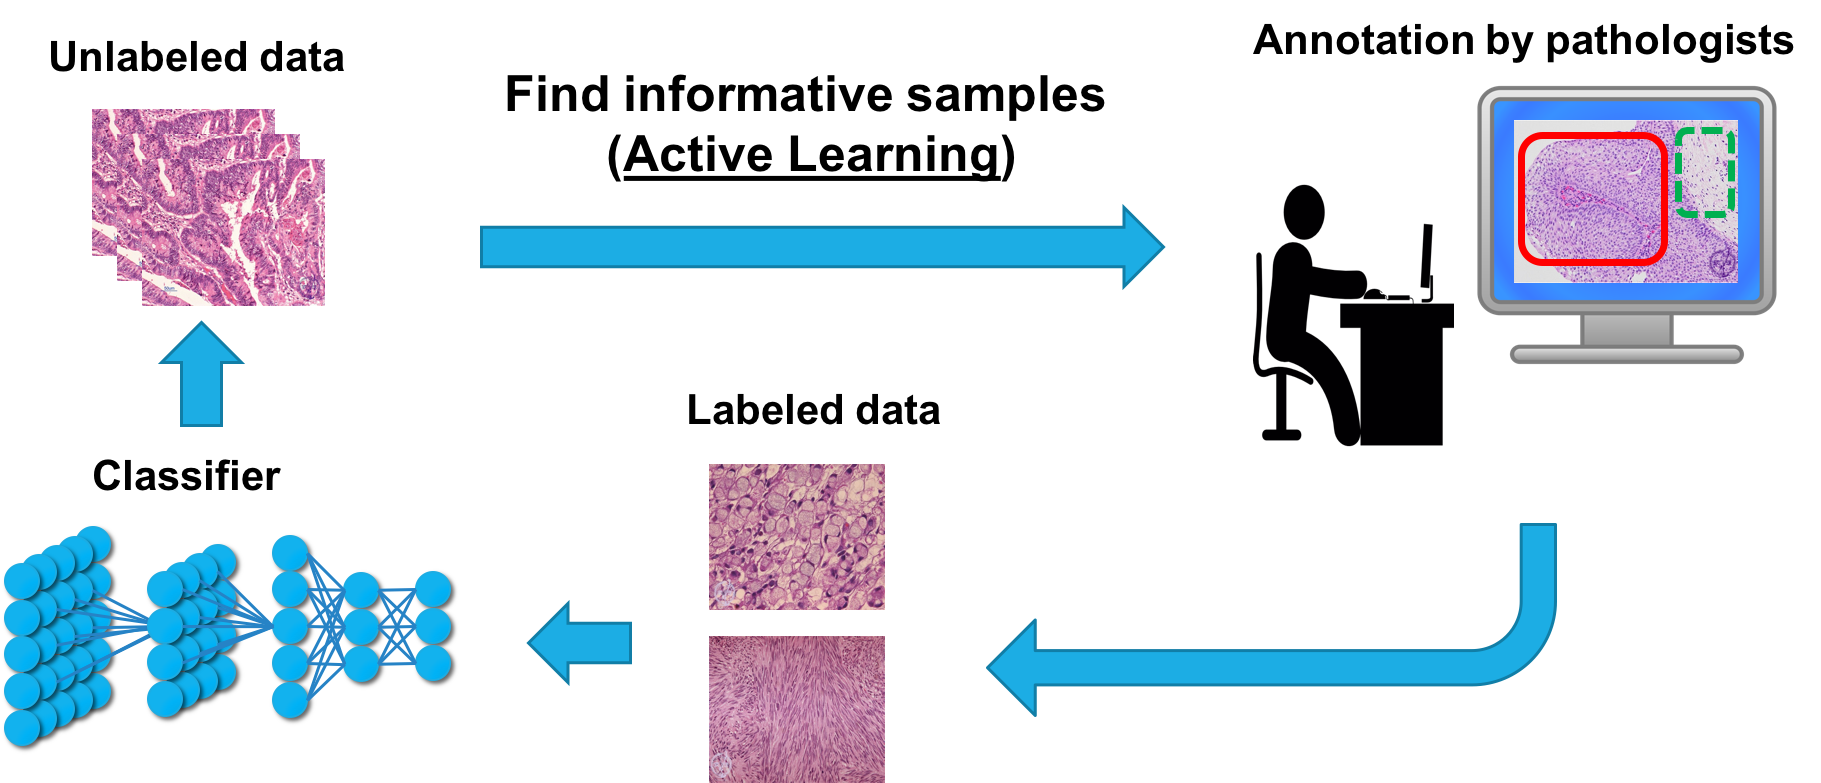
\includegraphics[width=120mm]{figures/overview.png}
     \end{center}
    \caption{本研究で提案するシステムの概念図}
\end{figure}

\section{Query by Dropout predictions}
ニューラルネットワークによって識別問題を解く際には、最終出力が各ラベルに対応する確率となるような確率分布を出力する。
しかし、前章で述べたように、ニューラルネットワーク自体のパラメータに対する不確かさをモデルしているわけではない。
このように不確かさを陽にモデル化しない識別器を利用した能動学習において、Query By Committeeはしばしば用いられる手法である。
しかし、ニューラルネットワークのように非常に計算コストの重いモデルを複数同時に保持し学習を行うことはメモリ、
計算時間等様々な問題で現実的ではないという問題があった。
そこで、本研究では、正則化に利用されるDropoutによって本体のネットワークからサンプリングされた
部分ネットワークをCommitteeとみなし、近似的にQuery-By-Committeeを行う手法を提案する。

\begin{figure}[tbp]
    \label{fig:query_by_dropout}
     \begin{center}
      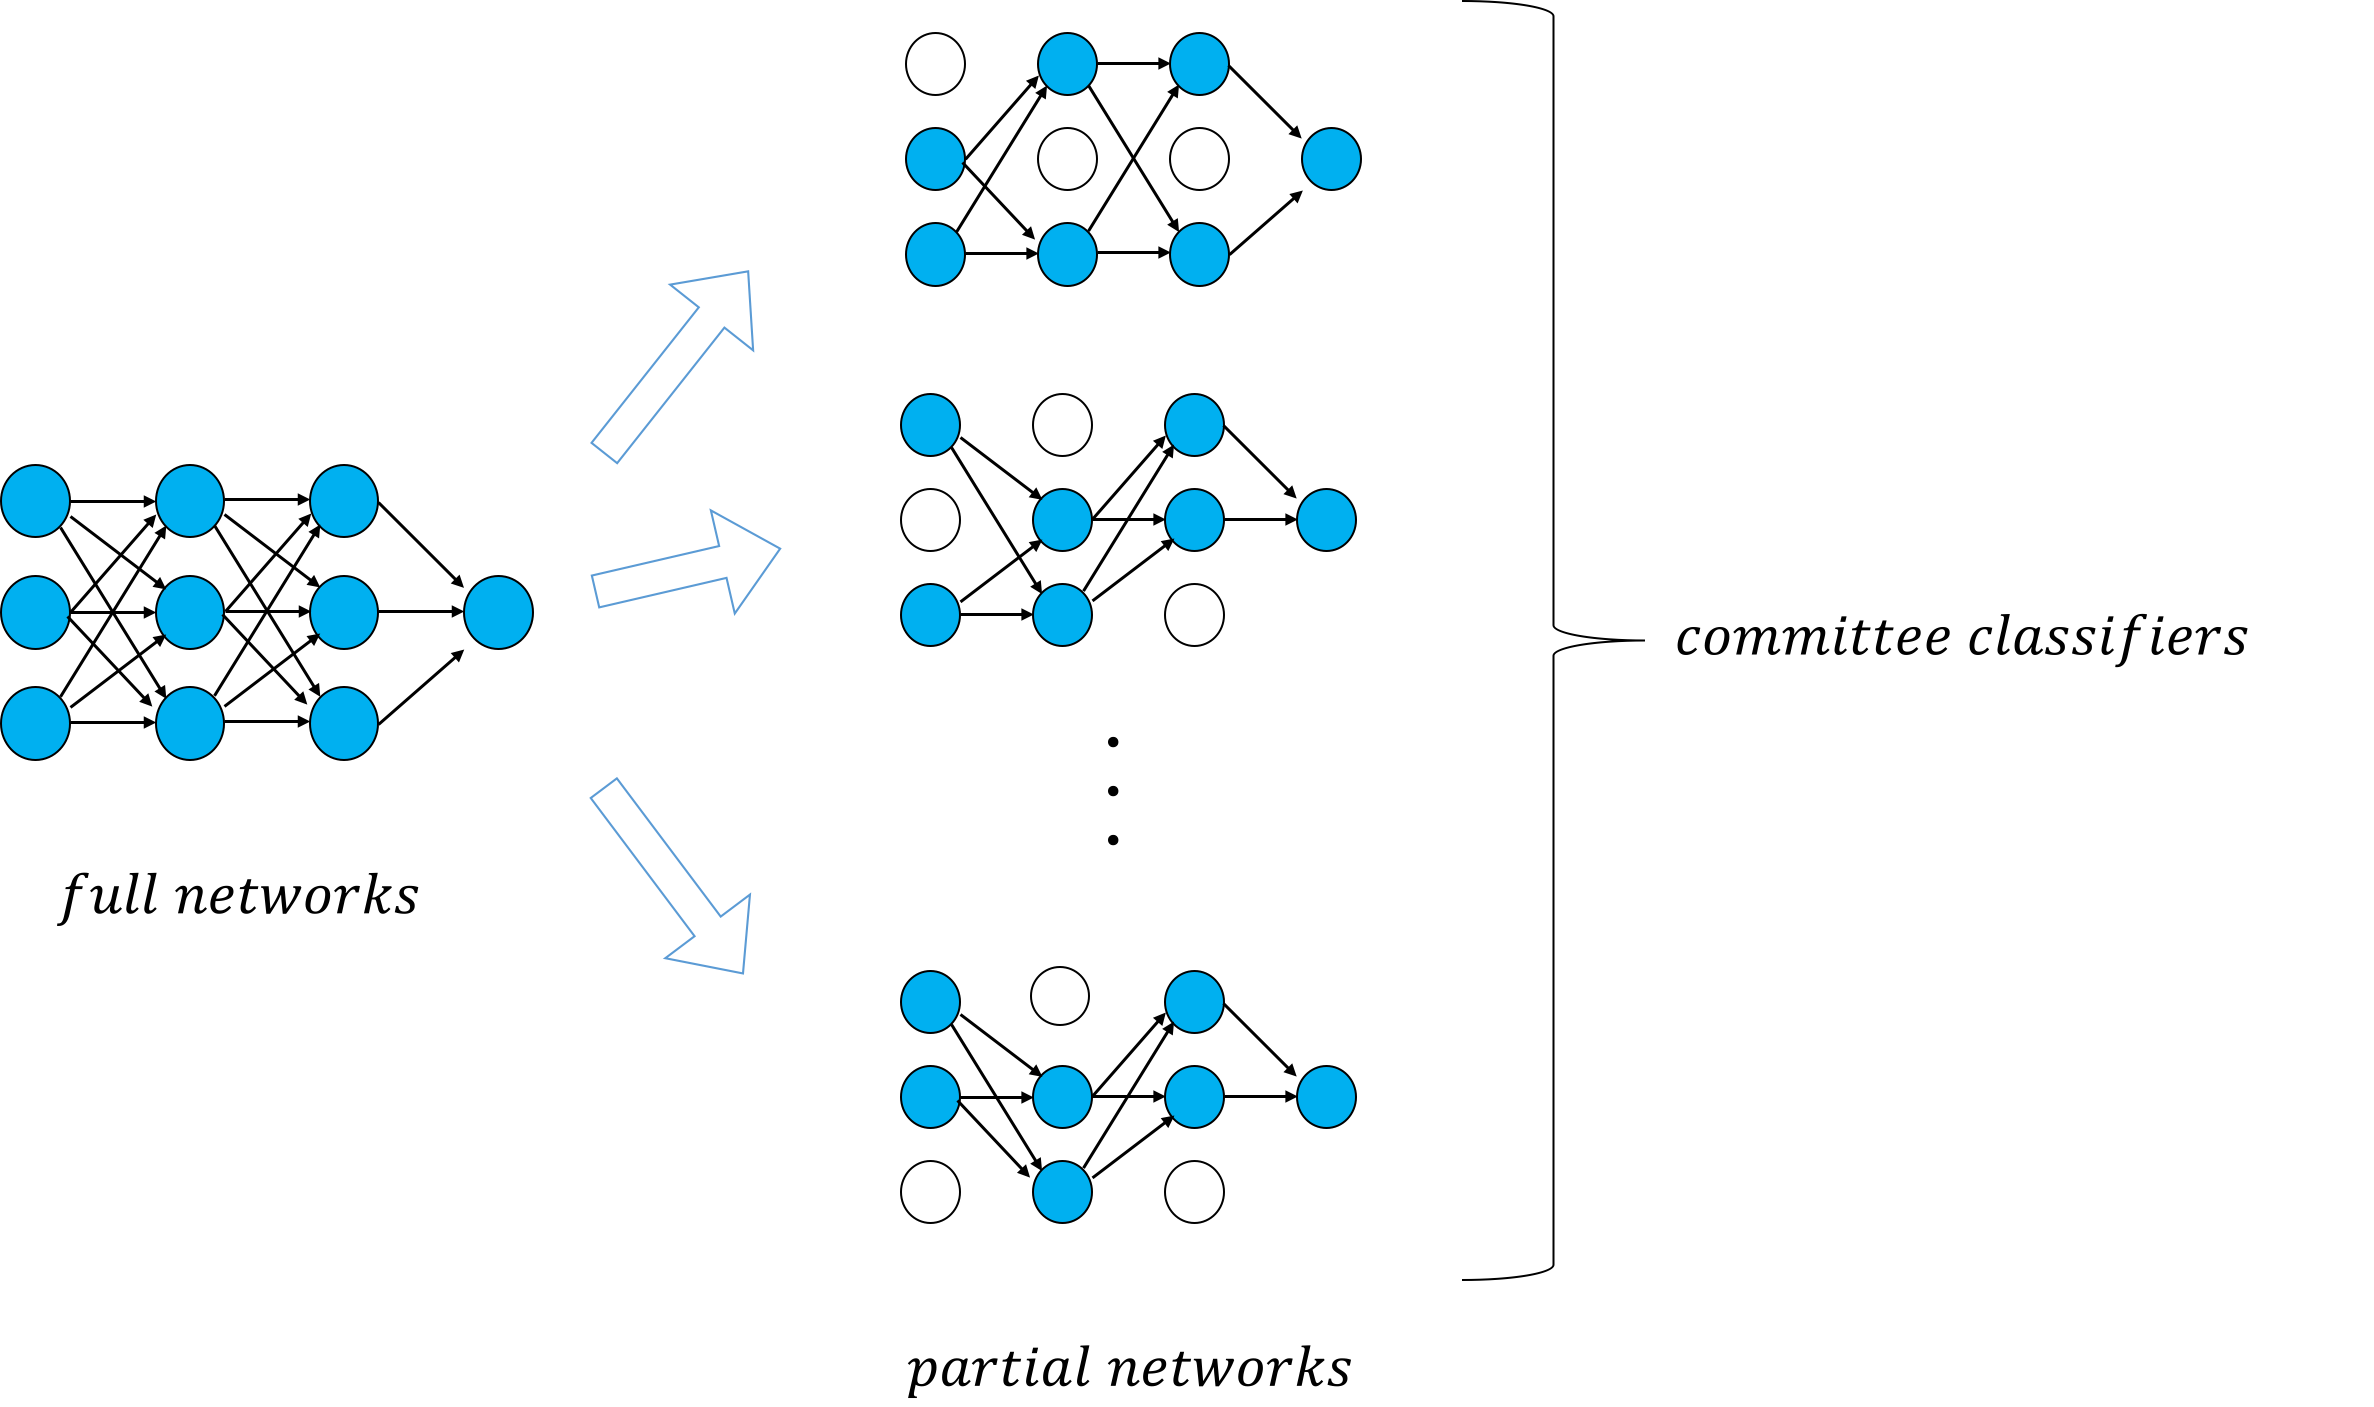
\includegraphics[width=120mm]{figures/query_by_dropout.png}
     \end{center}
    \caption{Dropoutによってサンプリングされた部分ネットワークによってCommitteeを形成する。}
\end{figure}

\subsection{Data Augmentation}

\subsection{理論的説明}



\section{バッチ型能動学習への拡張}
深層学習器を能動学習に利用する場合、1iteration毎に計算コストがかかってしまうため、
各クエリ問い合わせにおいて複数のサンプルにラベリングを付与してもらうバッチ型能動学習を採用するのが適当であると考えられる。
一度に投げるクエリ内で情報の重複が起きないようにするためには何らかの工夫をする必要があるが、
2章で述べたような劣モジュラ関数を設計するのは深層学習を利用する場合計算コストの観点から難しい。
そこで、本研究ではクラスタリングにより同一のクラスターに属するサンプルは2つ以上選択しないとすることで、情報の重複を避ける。
また、クラスタリングに使用する特徴量の候補として、以下の3つを考慮した。

\subsubsection{hand-crafted feature}
2章で述べたように、病理画像解析にはテクスチャ解析で用いられる技術がしばしば使用される。
ここでは、Local Binary Pattern (LBP)を採用する。

\subsubsection{CNNの中間特徴量}
Imagenetで学習された特徴量は様々なタスクに有用であるとされている。
そこで本研究ではGoogleNetの中間特徴量を利用した。

\subsubsection{Compact Bilinear Poolingによる特徴量}
近年の深層学習を用いたテクスチャ解析の研究で、Bilinear Poolingによって空間情報をなくした特徴量がしばしば利用される。
これは、CNNの中間特徴量の相関行列を計算し空間方向に平均を取ったものである。
\begin{eqnarray}
G_{ij} = \sum_k{F_{ik} F_{jk}}
\end{eqnarray}
また、一般にCNNの特徴量次元(チャンネル数)は256~512の大きな値であるため、そのまま計算した場合非常に高次元な値となってしまう。
そこで、その近似手法であるCompact Bilinear Pooling\cite{gao2016compact}を本研究ではCNNを用いたテクスチャ特徴量として採用する。

\section{まとめ}
